\documentclass{article}\usepackage[]{graphicx}\usepackage[]{color}
%% maxwidth is the original width if it is less than linewidth
%% otherwise use linewidth (to make sure the graphics do not exceed the margin)
\makeatletter
\def\maxwidth{ %
  \ifdim\Gin@nat@width>\linewidth
    \linewidth
  \else
    \Gin@nat@width
  \fi
}
\makeatother

\definecolor{fgcolor}{rgb}{0.345, 0.345, 0.345}
\newcommand{\hlnum}[1]{\textcolor[rgb]{0.686,0.059,0.569}{#1}}%
\newcommand{\hlstr}[1]{\textcolor[rgb]{0.192,0.494,0.8}{#1}}%
\newcommand{\hlcom}[1]{\textcolor[rgb]{0.678,0.584,0.686}{\textit{#1}}}%
\newcommand{\hlopt}[1]{\textcolor[rgb]{0,0,0}{#1}}%
\newcommand{\hlstd}[1]{\textcolor[rgb]{0.345,0.345,0.345}{#1}}%
\newcommand{\hlkwa}[1]{\textcolor[rgb]{0.161,0.373,0.58}{\textbf{#1}}}%
\newcommand{\hlkwb}[1]{\textcolor[rgb]{0.69,0.353,0.396}{#1}}%
\newcommand{\hlkwc}[1]{\textcolor[rgb]{0.333,0.667,0.333}{#1}}%
\newcommand{\hlkwd}[1]{\textcolor[rgb]{0.737,0.353,0.396}{\textbf{#1}}}%
\let\hlipl\hlkwb

\usepackage{framed}
\makeatletter
\newenvironment{kframe}{%
 \def\at@end@of@kframe{}%
 \ifinner\ifhmode%
  \def\at@end@of@kframe{\end{minipage}}%
  \begin{minipage}{\columnwidth}%
 \fi\fi%
 \def\FrameCommand##1{\hskip\@totalleftmargin \hskip-\fboxsep
 \colorbox{shadecolor}{##1}\hskip-\fboxsep
     % There is no \\@totalrightmargin, so:
     \hskip-\linewidth \hskip-\@totalleftmargin \hskip\columnwidth}%
 \MakeFramed {\advance\hsize-\width
   \@totalleftmargin\z@ \linewidth\hsize
   \@setminipage}}%
 {\par\unskip\endMakeFramed%
 \at@end@of@kframe}
\makeatother

\definecolor{shadecolor}{rgb}{.97, .97, .97}
\definecolor{messagecolor}{rgb}{0, 0, 0}
\definecolor{warningcolor}{rgb}{1, 0, 1}
\definecolor{errorcolor}{rgb}{1, 0, 0}
\newenvironment{knitrout}{}{} % an empty environment to be redefined in TeX

\usepackage{alltt}
\usepackage[sc]{mathpazo}
\renewcommand{\sfdefault}{lmss}
\renewcommand{\ttdefault}{lmtt}
\usepackage[T1]{fontenc}
\usepackage{geometry}
\geometry{verbose,tmargin=2.5cm,bmargin=2.5cm,lmargin=2.5cm,rmargin=2.5cm}
\setcounter{secnumdepth}{2}
\setcounter{tocdepth}{2}
\usepackage[unicode=true,pdfusetitle,
 bookmarks=true,bookmarksnumbered=true,bookmarksopen=true,bookmarksopenlevel=2,
 breaklinks=false,pdfborder={0 0 1},backref=false,colorlinks=false]
 {hyperref}
\hypersetup{
 pdfstartview={XYZ null null 1}}

\makeatletter
%%%%%%%%%%%%%%%%%%%%%%%%%%%%%% User specified LaTeX commands.
\renewcommand{\textfraction}{0.05}
\renewcommand{\topfraction}{0.8}
\renewcommand{\bottomfraction}{0.8}
\renewcommand{\floatpagefraction}{0.75}

\makeatother
\IfFileExists{upquote.sty}{\usepackage{upquote}}{}
\begin{document}








The results below are generated from an R script.

\begin{knitrout}
\definecolor{shadecolor}{rgb}{0.969, 0.969, 0.969}\color{fgcolor}\begin{kframe}
\begin{alltt}
\hlcom{#R Code for Lab 3}
\hlcom{#Jan Domingo}


\hlcom{#1A: Generate 10,000 variates using the random number generator}
\hlcom{#Generate random variates according to the RANDU generator}
\hlcom{#X_(n+1) = 16807 X_n mod 2^31; a = 16807, c = 0, m = 2^31-1}
\hlstd{n} \hlkwb{=} \hlnum{10000} \hlcom{#number of variates}
\hlstd{x} \hlkwb{=} \hlnum{1} \hlcom{#seed}
\hlkwa{for} \hlstd{(i} \hlkwa{in} \hlnum{1}\hlopt{:}\hlstd{n) \{}
  \hlstd{x} \hlkwb{=} \hlkwd{c}\hlstd{(x, (}\hlnum{16807}\hlopt{*}\hlstd{x[i])}\hlopt\hlstd{(}\hlnum{2}\hlopt{^}\hlnum{31}\hlopt{-}\hlnum{1}\hlstd{))} \hlcom{#modulus}
\hlstd{\}}
\hlstd{x} \hlkwb{=} \hlstd{x[}\hlnum{2}\hlopt{:}\hlstd{(n}\hlopt{+}\hlnum{1}\hlstd{)]} \hlcom{#Disregards seed value, keeps the other 10000 from for loop}
\hlstd{u} \hlkwb{=} \hlstd{x}\hlopt{/}\hlstd{(}\hlnum{2}\hlopt{^}\hlnum{31}\hlopt{-}\hlnum{1}\hlstd{)}  \hlcom{#Transforming uniform variates between 0 and 1}


\hlcom{#1B: Draw a historgram of these variates}
\hlkwd{par}\hlstd{(}\hlkwc{mfrow} \hlstd{=} \hlkwd{c}\hlstd{(}\hlnum{2}\hlstd{,}\hlnum{1}\hlstd{))} \hlcom{#2 rows, 1 column for the graph matrix}
\hlkwd{hist}\hlstd{(u,} \hlkwc{main}\hlstd{=}\hlstr{""}\hlstd{,} \hlkwc{xlab} \hlstd{=} \hlstr{"RANDU variates"}\hlstd{,} \hlkwc{ylab} \hlstd{=} \hlstr{"Frequencies"}\hlstd{)} \hlcom{# histogram of the n RANDU variates}


\hlcom{#1C: Draw the empirical cumulative distribution function against the CDF}
\hlkwd{plot.ecdf}\hlstd{(u,} \hlkwc{verticals} \hlstd{=} \hlnum{TRUE}\hlstd{,} \hlkwc{do.p} \hlstd{=} \hlnum{FALSE}\hlstd{,} \hlkwc{main}\hlstd{=}\hlstr{""}\hlstd{,} \hlkwc{ylab} \hlstd{=} \hlstr{"Probability"}\hlstd{)}
\hlkwd{abline}\hlstd{(}\hlnum{0}\hlstd{,}\hlnum{1}\hlstd{,} \hlkwc{col}\hlstd{=}\hlstr{"red"}\hlstd{)}
\end{alltt}
\end{kframe}

{\centering 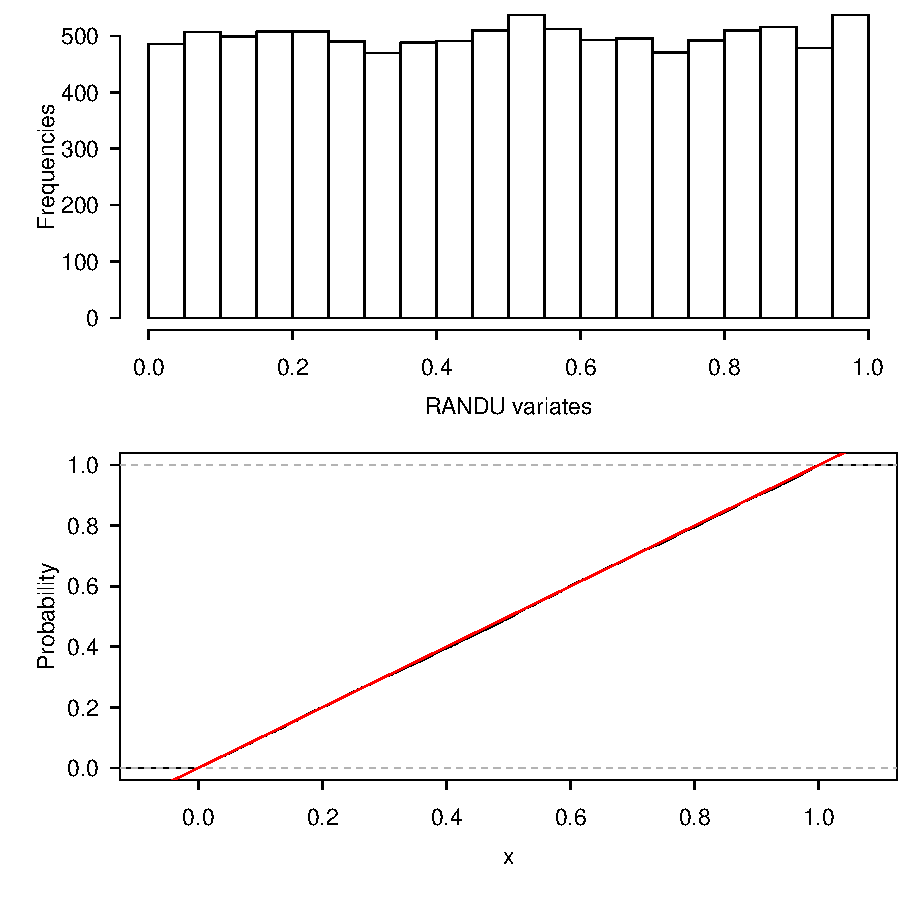
\includegraphics[width=.6\linewidth]{figure/lab3code-Rnwauto-report-1} 

}


\begin{kframe}\begin{alltt}
\hlcom{#1D: Kolmogorov-Smirnov Test of RANDU variates against U(0, 1) distribution}
\hlkwd{ks.test}\hlstd{(u,} \hlstr{"punif"}\hlstd{,} \hlnum{0}\hlstd{,} \hlnum{1}\hlstd{)}
\end{alltt}
\begin{verbatim}
## 
## 	One-sample Kolmogorov-Smirnov test
## 
## data:  u
## D = 0.0070995, p-value = 0.6946
## alternative hypothesis: two-sided
\end{verbatim}
\begin{alltt}
\hlcom{#2B:Calculates the EPMF and the ECDF }
\hlstd{n} \hlkwb{=} \hlnum{1000}
\hlstd{x} \hlkwb{=} \hlnum{0} \hlcom{#initial vector)}
\hlstd{bpmf} \hlkwb{=} \hlkwd{rep}\hlstd{(}\hlnum{0.20}\hlstd{,} \hlnum{5}\hlstd{)} \hlcom{#True PMF}
\hlstd{bcdf} \hlkwb{=} \hlkwd{cumsum}\hlstd{(bpmf)} \hlcom{#True CDF}
\hlstd{uniLine} \hlkwb{=} \hlkwd{c}\hlstd{(}\hlnum{0}\hlstd{,bcdf)} \hlcom{#Uniform line from 0-1 broken into 4 intervals}
\hlstd{xval} \hlkwb{=} \hlnum{1}\hlopt{:}\hlnum{5} \hlcom{#1 = S, 2 = L, 3 = U, 4 = R, 5 = M}
\hlkwa{for} \hlstd{(i} \hlkwa{in} \hlnum{1}\hlopt{:}\hlstd{n) \{}
  \hlstd{u} \hlkwb{=} \hlkwd{runif}\hlstd{(}\hlnum{1}\hlstd{)}  \hlcom{#Sample a random variate from U(0,1). The inverse transofrmation method}
  \hlstd{x[i]} \hlkwb{=} \hlkwd{sum}\hlstd{(u} \hlopt{>} \hlstd{uniLine)} \hlcom{#Random variate between 1 and 5 (letter on bottle cap) }
\hlstd{\}}
\hlstd{epmf} \hlkwb{=} \hlkwd{table}\hlstd{(x)}\hlopt{/}\hlstd{n} \hlcom{#Emprical PMF}
\hlstd{ecdf} \hlkwb{=} \hlkwd{cumsum}\hlstd{(epmf)} \hlcom{#Empirical CDF}


\hlcom{#2C: Present a histogram of your variates}
\hlkwd{hist}\hlstd{(x,} \hlkwc{xlab}\hlstd{=}\hlstr{"Bottle Cap Letter"}\hlstd{,} \hlkwc{ylab}\hlstd{=}\hlstr{"Frequencies"}\hlstd{,} \hlkwc{breaks}\hlstd{=}\hlkwd{seq}\hlstd{(}\hlkwd{min}\hlstd{(x)}\hlopt{-}\hlnum{0.5}\hlstd{,} \hlkwd{max}\hlstd{(x)}\hlopt{+}\hlnum{0.5}\hlstd{))}


\hlcom{#2D: Present a plot of the emprical cdf versues the true cdf}
\hlkwd{plot}\hlstd{(xval, bcdf,} \hlkwc{xlab}\hlstd{=}\hlstr{"Letter"}\hlstd{,} \hlkwc{yLab}\hlstd{=}\hlstr{"CDF"}\hlstd{,} \hlkwc{main}\hlstd{=}\hlstr{"ECDF vs True CDF"}\hlstd{,} \hlkwc{pch}\hlstd{=}\hlnum{19}\hlstd{)}
\end{alltt}


{\ttfamily\noindent\color{warningcolor}{\#\# Warning in plot.window(...): "{}yLab"{} is not a graphical parameter}}

{\ttfamily\noindent\color{warningcolor}{\#\# Warning in plot.xy(xy, type, ...): "{}yLab"{} is not a graphical parameter}}

{\ttfamily\noindent\color{warningcolor}{\#\# Warning in axis(side = side, at = at, labels = labels, ...): "{}yLab"{} is not a graphical parameter}}

{\ttfamily\noindent\color{warningcolor}{\#\# Warning in axis(side = side, at = at, labels = labels, ...): "{}yLab"{} is not a graphical parameter}}

{\ttfamily\noindent\color{warningcolor}{\#\# Warning in box(...): "{}yLab"{} is not a graphical parameter}}

{\ttfamily\noindent\color{warningcolor}{\#\# Warning in title(...): "{}yLab"{} is not a graphical parameter}}\begin{alltt}
\hlkwd{points}\hlstd{(xval, ecdf,} \hlkwc{pch}\hlstd{=}\hlnum{8}\hlstd{,} \hlkwc{col}\hlstd{=}\hlstr{"red"}\hlstd{)}
\end{alltt}
\end{kframe}

{\centering 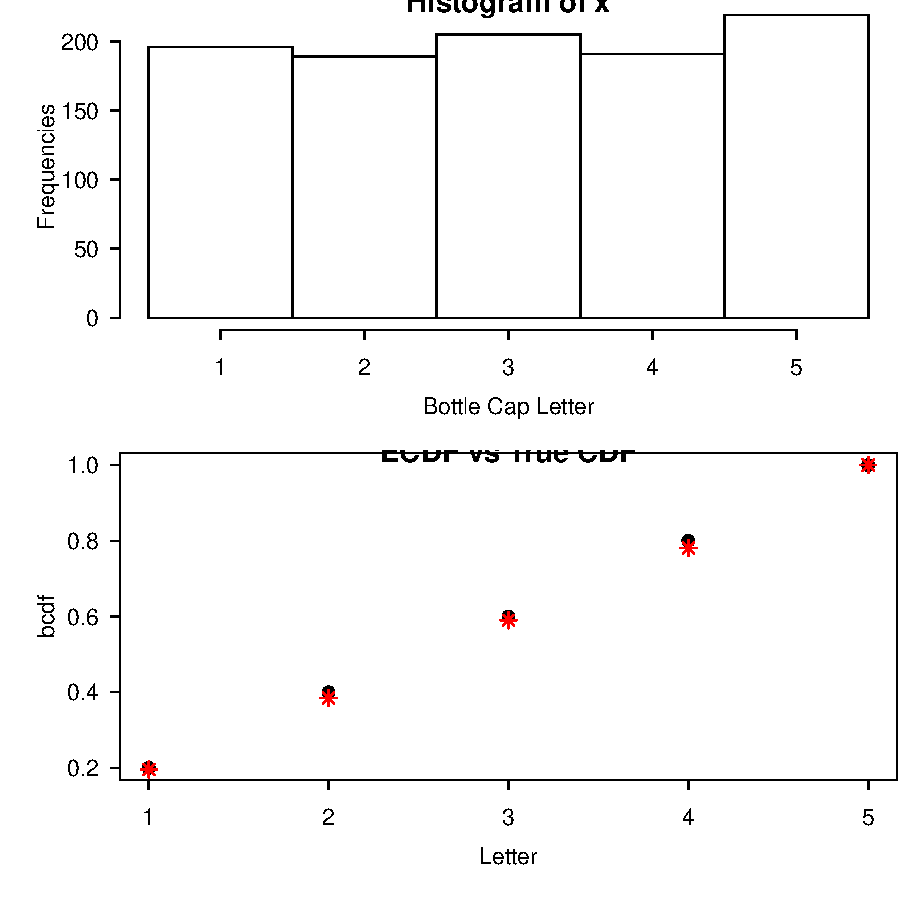
\includegraphics[width=.6\linewidth]{figure/lab3code-Rnwauto-report-2} 

}



\end{knitrout}

The R session information (including the OS info, R version and all
packages used):

\begin{knitrout}
\definecolor{shadecolor}{rgb}{0.969, 0.969, 0.969}\color{fgcolor}\begin{kframe}
\begin{alltt}
\hlkwd{sessionInfo}\hlstd{()}
\end{alltt}
\begin{verbatim}
## R version 3.5.2 (2018-12-20)
## Platform: x86_64-apple-darwin15.6.0 (64-bit)
## Running under: macOS Mojave 10.14.3
## 
## Matrix products: default
## BLAS: /System/Library/Frameworks/Accelerate.framework/Versions/A/Frameworks/vecLib.framework/Versions/A/libBLAS.dylib
## LAPACK: /Library/Frameworks/R.framework/Versions/3.5/Resources/lib/libRlapack.dylib
## 
## locale:
## [1] en_US.UTF-8/en_US.UTF-8/en_US.UTF-8/C/en_US.UTF-8/en_US.UTF-8
## 
## attached base packages:
## [1] stats     graphics  grDevices utils     datasets  methods   base     
## 
## other attached packages:
## [1] knitr_1.22
## 
## loaded via a namespace (and not attached):
## [1] compiler_3.5.2 magrittr_1.5   tools_3.5.2    stringi_1.4.3  highr_0.7     
## [6] stringr_1.4.0  xfun_0.5       evaluate_0.13
\end{verbatim}
\begin{alltt}
\hlkwd{Sys.time}\hlstd{()}
\end{alltt}
\begin{verbatim}
## [1] "2019-04-30 15:06:14 PDT"
\end{verbatim}
\end{kframe}
\end{knitrout}


\end{document}
